\label{desenvolvimento}

%Escrever o que será apresentado no capítulo
Neste capítulo serão apresentados ao que se propõe o framework e como ele será trabalhado, como foi realizado o desenvolvimento da ferramenta, como é a interface que será apresentada ao usuário, a forma de se utilizar os cards no sistema e como eles podem ser editados para adequações futuras em outras propostas de frameworks para elicitação de requisitos em ética em \acrshort{IA}.

\section{Proposta}

A ferramenta a ser desenvolvida neste trabalho servirá como um assistente para os Product Owners e desenvolvedores elicitarem requisitos éticos em sistemas baseados em IA durante a primeira fase do ciclo de desenvolvimento de software e a análise de requisitos, no contexto de desenvolvimento ágil de software. Para esta fase de discussão, será utilizado um formato de \textit{Planning Poker} digital, com acesso disponível \href{https://oggvaldo.github.io/eccola}{no repositório no GitHub}

Será implementada um método desenvolvido por Vakkuri et al. \cite{ECCOLA} denominado ECCOLA, onde os autores conceberam um baralho de cartas com questões éticas a serem debatidas pela a equipe de desenvolvimento.

A implementação das cartas de papel em uma interface gráfica se justifica no contexto de trabalho remoto devido a pandemia do COVID-19, além de prover um meio adequado para que pesquisadores possam avaliar a ferramenta de maneira mais automatizada.

Ademais, o modelo adotado de planning poker propõe uma discussão de forma mais lúdico, de fácil entendimento e praticidade, uma vez que a ferramenta poderá ser acessada tanto por dispositivos móveis (\textit{smartphones} e \textit{tablets}) quanto computadores (\textit{desktops} e \textit{notebooks}).

\section{Desenvolvimento}

Para o desenvolvimento deste sistema, foram utilizadas as tecnologias de \textit{Hypertext Markup Language} \acrshort{HTML} \cite{HTMLsite}, \textit{Cascading Style Sheets} \acrshort{CSS} \cite{CSSsite} e JavaScript \acrshort{JS} \cite{JavaScriptsite}. Para a apresentação da página inicial e a página que vai apresentar as cartas, temos o \acrshort{HTML} como a base, o \acrshort{CSS} como a parte de estilização da página, além de fornecer padrões adaptivos para diversos tamanhos de tela, manutenabilidade e escalabilidade visual do programa sem a necessidade de ferramentas e \textit{frameworks} adicionais, e o \acrshort{JS} como a parte responsável pela lógica e ação de funcionalidades do sistema. Com este conjunto de ações, teremos aqui o que será um tipo de aplicação web, uma aplicação que funcionará diretamente do navegador de qualquer dispositivo com capacidade computacional e que seja compatível com HTML 5 \cite{webapp}.

Com isso, temos um sistema totalmente responsivo a diversos tamanhos de tela. Isto permite seu uso em dispositivos como \textit{smartphones}, \textit{tablets}, \textit{notebooks} e computadores de mesa. Temos esta possibilidade graças ao uso de \textit{Media Queries} do CSS empregado, que nos deixa realizar a apresentação do conteúdo de forma adaptiva a cada um dos dispositivos supracitados, sem precisar realizar alterações específicas para cada um dos tipos de equipamentos e/ou telas.

Durante a criação deste guia, alguns cuidados foram tomados. O \acrshort{HTML} foi criado de forma a permitir a legibilidade e compreensibilidade com o uso devido do \acrshort{HTML} semântico (por exemplo, como as tags semânticas identificam o conteúdo que se encontra nos arquivos do sistema), deixando assim a leitura do código de forma mais sucinta e de mais fácil identificação. Além disto, o sistema foi pensado também a ser usado por pessoas com deficiência visual graças ao uso de tal técnica. Para tanto, este sistema está perfeitamente adaptado ao uso de sistemas ledores de tela, como o \href{https://www.nvaccess.org/}{\textit{Non Visual Desktop Access} (NVDA)}.

Juntamente com a disponibilização de um site estático com o uso do \acrshort{HTML} e do \acrshort{CSS}, o \acrshort{JS} foi usado para trazer ao sistema os elementos que fornecem a interatividade e o dinamismo do sistema para os usuários. Assim, foi possível dar ao usuário as possibilidades de seleção e comparação das cartas, filtragem de acordo o princípio ético que pretendem explorar e a facilidade na realização de alterações do sistema para outros tipos de elicitações a serem inseridos no sistema, trazendo assim a quem tem um conhecimento de lógica de programação também as possibilidades de modificar e adicionar cartas e princípios éticos sem grandes dificuldades, tudo visando um sistema para ser o mais \textit{user-friendly}, tanto para quem vier o operar quanto para quem vier editar o sistema através do livre download do repositório localizado no  \href{https://www.github.com/oggvaldo/eccola}{repositório} em que o sistema se encontra disponível.

Com isso, temos em mente o objetivo de contemplar os princípios éticos encontrados na área de ética em IA com o fornecimento do sistema e de seu código-fonte, compreensibilidade e instruções de uso explorando o princípio ético da transparência, com foco nas questões éticas de divulgação, comunicação, apresentação, explicabilidade, compreensibilidade e interpretabilidade, e ao adequar a tecnologia para o uso de \textit{softwares} leitores de tela temos a contemplação do princípio de beneficência e dignidade atendidos segundo os princípios éticos definidos por Ryan e Stahl \cite{Ryan2020ArtificialIE}.

Com todos os aspectos técnicos de software descritos anteriormente, na entrada do sistema o usuário poderá ler como se utiliza as cartas em um contexto de desenvolvimento ágil com o uso da técnica de \textit{planning poker}, conforme a figuras abaixo apresentam.

\begin{figure}[h!]
    \centering
    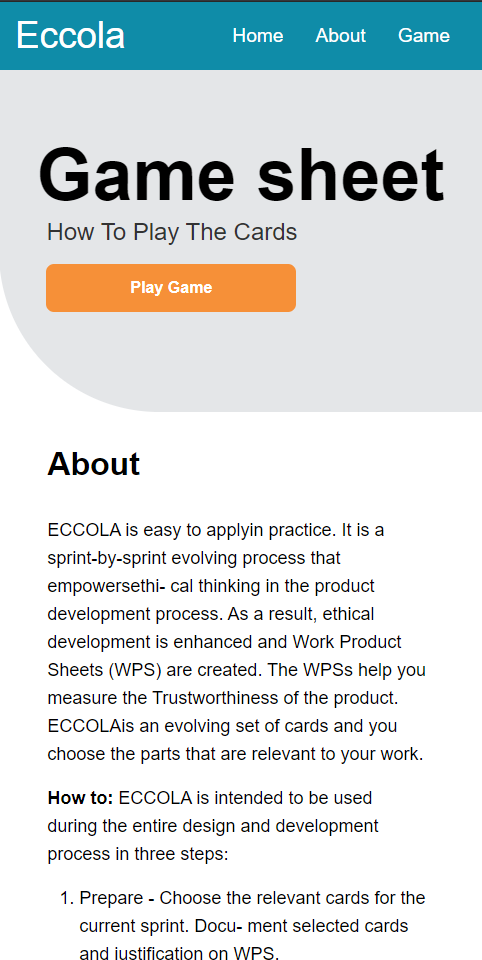
\includegraphics[width=0.3\textwidth]{img/eccola_celular.png}
    \caption{Imagem do sistema adaptado para telas de \textit{smartphones} e \textit{tablets}}
    \label{fig:eccola_celular}
\end{figure}

\begin{figure}[h!]
    \centering
    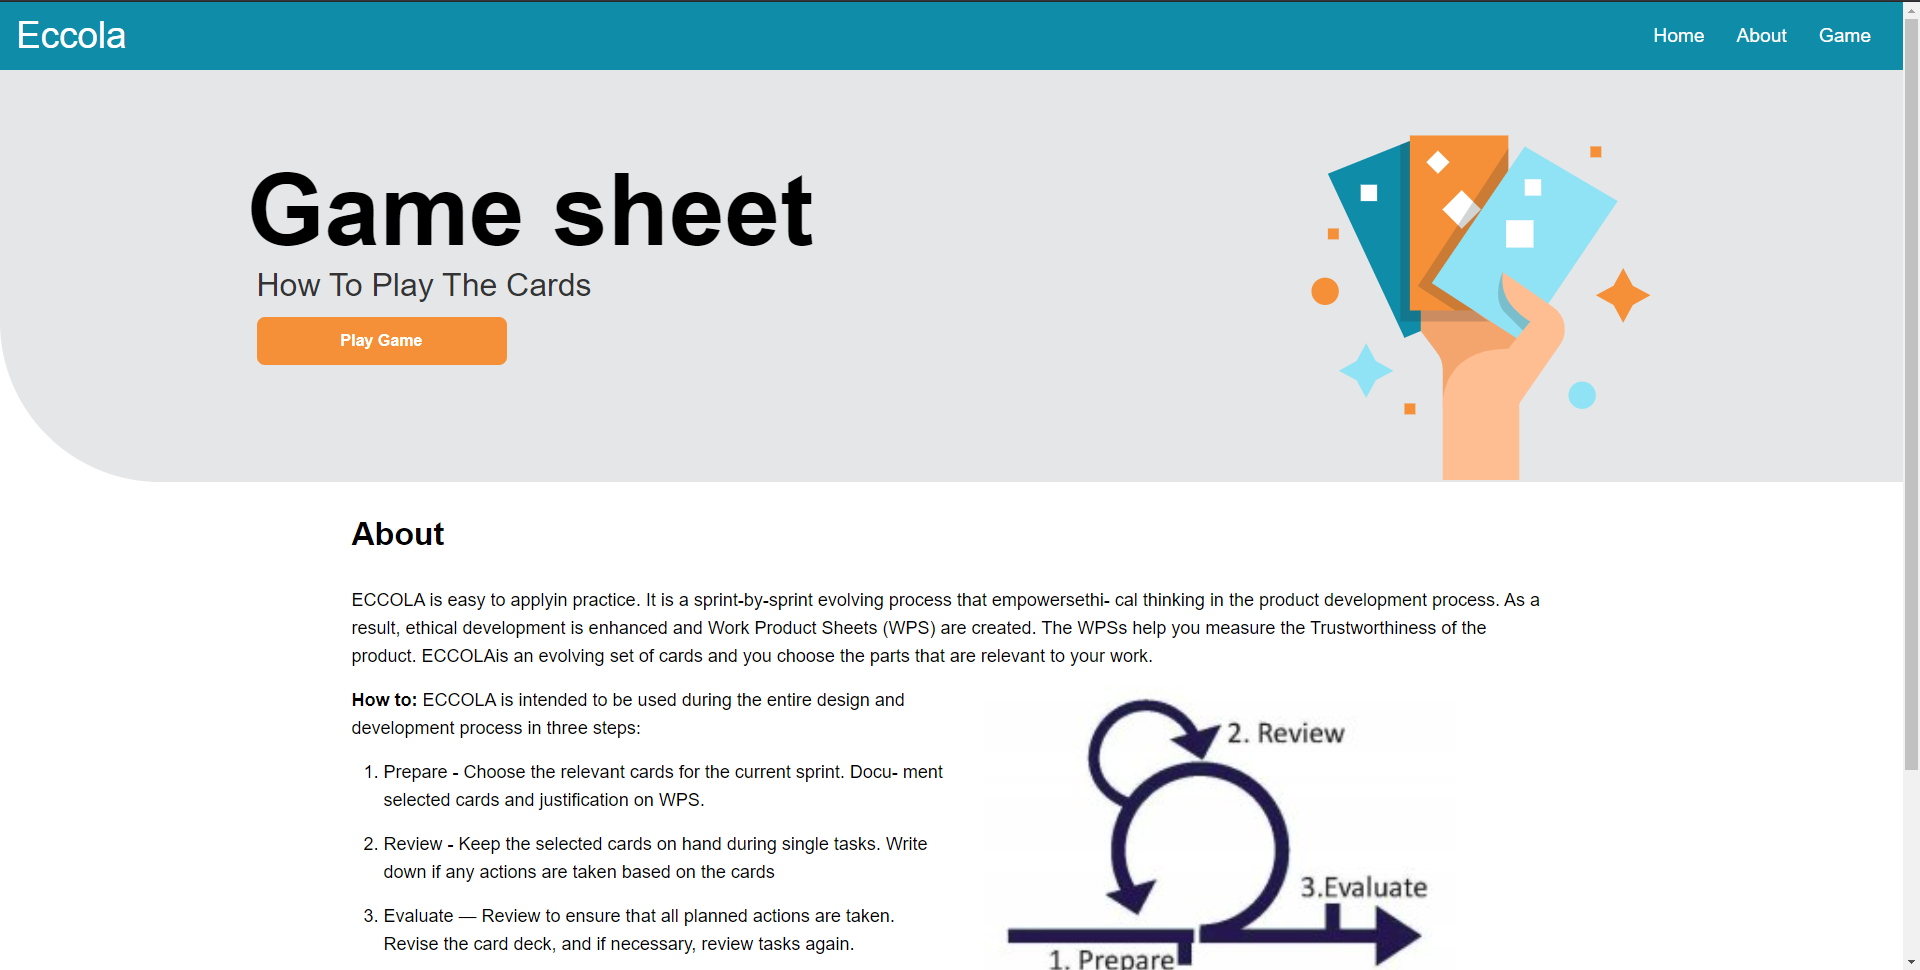
\includegraphics[width=0.6\textwidth]{img/eccola_desktop.png}
    \caption{Imagem do sistema adaptado para telas de computadores de mesa e \textit{notebooks}.}
    \label{fig:eccola_desktop}
\end{figure}

\subsection{Interface}


% Explicar porque os cards foram criados, como o CSS foi essencial nesta parte e como o conceito de Planning poker ajudou a estruturar o guia de elicitações.

\section{Como utilizar}
Explicar como se dá a utilização do sistema, no que ele pode ser útil para o discussão da elicitação de requisitos de IA, usando como base o ECCOLA e seu uso de inspiração de framework. 
\subsection{Utilizando os \textit{cards}}
Excplicar como o conceito de planning poker será aplicado com a discussão nas elicitações de requisito, como a seleção de cartas e sua posterior discussão podem definir para os guias delimitados pelo eccola mas também mostrar como baseado em ryan e stahl qualquer outro princípio para a elicitação de requisitos em ética em IA também pode ser aplicado com este guia-base.
\subsection{Editando os \textit{cards}}
Além da inserção de parte do código-fonte de como as cartas foram estruturadas, o que cada campo pode fazer e como cada campo pode ser alterado após criar um fork do projeto no github para adequação de guias futuros a serem desenvolvidos por quem se interessar.
% Inserir snippet codigo de carta